\documentclass{article}
\usepackage{polski}
\usepackage[utf8]{inputenc}
\usepackage{graphicx}
\usepackage{placeins}
\usepackage{siunitx}
\sisetup{math-micro=\text{µ},text-micro=µ}
\graphicspath{ {./img/} }

\title{Regresja liniowa i drzewa decyzyjne}
\author{Piotr Kumala}
\date{06.06.2022 r.}

\begin{document}
	
	\maketitle
	
	\section{Wstęp}
	W tym dokumencie przedstawione zostanie zastosowanie klasycznych metod predykcji szeregów czasowych, ich wyniki oraz wnioski z nich płynące. Uzyskane wyniki zostaną wykorzystane jako wartości referencyjne przy analizie skuteczności zastosowań rekurencyjnych sieci neuronowych do tego samego problemu. W podsumowaniu przedstawiony zostanie również dalszy kierunek prowadzonych prac oraz ostateczny cel tychże badań. 
	
	\section{Wybór danych do dalszej analizy}
	W trakcie przeprowadzania regresji liniowej zauważono, że przygotowany wcześniej zbiór danych o wypadkach rowerowych w Wielkiej Brytanii niestety nie jest odpowiedni do przeprowadzania na nim predykcji. Każdy wypadek posiada informacje o warunkach pogodowych, oświetleniu, porze dnia i rodzaju drogi. Nie można jednak na podstawie żadnej z tych charakterystyk prowadzić wnioskowania o ilości wypadków danego dnia. Nie został przygotowany szereg czasowy opisujący te cechy, a stworzenie go jest bardzo skomplikowane o ile w ogóle wykonalne. 
	Z tego powodu podjęta została decyzja o porzuceniu tych danych i skupieniu dalszej pracy nad danymi klimatyczno-pogodowymi Krakowa w latach 2000-2021. W pracy nad tymi danymi nie zauważono żadnych znaczących problemów i wydaje się, że są one odpowiednie do prowadzenia dalszych badań. 
	
	
	\section{Regresja liniowa}
	Przeprowadzona została regresja liniowa gdzie na podstawie minimalnej temperatury gruntu, dziennej sumy opadów oraz maksymalnej, minimalnej i średniej dziennej temperatury estymowana była średni dzienny poziom zanieczyszczenia pyłem PM10. 
	
	Dane zostały podzielone na zbiory trenujący i testujący, a następnie przeprowadzona została najprostsza regresja liniowa. W jej wyniku otrzymaliśmy błąd średniokwadratowy równy 1386.2897378586617 $\frac{\si{\micro\gram}}{\si\meter^3}$ oraz wynik testu $R^2$ równy 0.323. Sporządzony został również wykres przewidywanego oraz rzeczywistego poziomu zanieczyszczenia pyłem PM10:
	\begin{figure}[!ht]
		\centering
		\makebox[0pt]{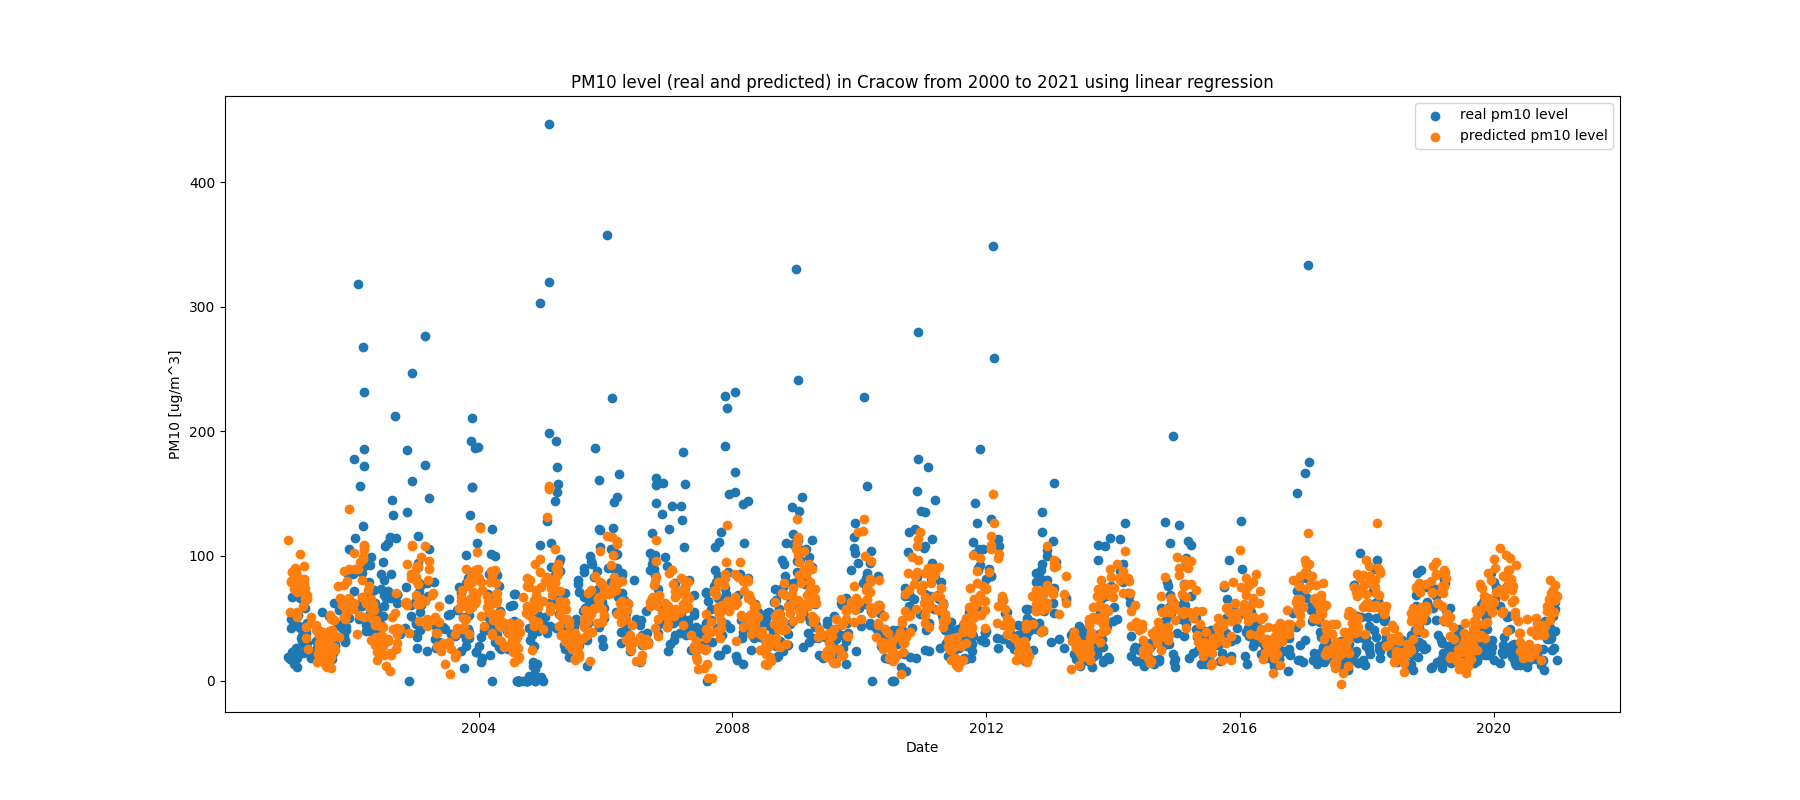
\includegraphics[scale=0.35]{linear_regression}}
		\caption{Wyniki regresji liniowej}
	\end{figure}
	\FloatBarrier
	\section{Drzewo decyzyjne}
	\section{Wnioski}
	
\end{document}